\section{Introduction}

%Imagine learning to perform any arbitrary simple task, like classifying a photograph as cat or not with knowing what a cat even is beforehand, by trying to correctly solve it repeatedly, over and over and over but every time on a completely new image of either a cat or not a cat. Failure to answer correctly will be punished. Moderate progress is made with each repetition as features such as whiskers, tails, ears, claws and texture are learned to be useful for correctly solving this task. There is a catch to learning in this manor, as it requires the examples of cat and not cats and someone that knows what a cat is has make these examples in the first place, , luckily internet search engines are around for us humans. Now take a much more complex task of correctly navigating a difficult three dimensional environment and picking an object with an robot arm, learning in the same fashion as the previously mentioned

%Physical robots suffer from the limitation of not being able to overcome physical constants of our universe as heat di, where as robots in simulated environment. 


Current state of the art in game engine, virtual reality and user-friendly development technologies allows for rapid prototyping of convincing environments, where in user can intuitively move around interact with objects. The Neodroid project strives to learn the user's intent from the user interacting with the environment. Once the intent is captured, a series of slightly differing simulations with the same intent can accelerate data collection, rather than the user tirelessly having to complete same intent repeatedly in only slightly differing environments. 
Once an agent has learned to replicate the intelligent behaviour and intent of the user through the use of the simulated data, it can explorer other possibly more efficient solution in a reinforcement learning environment.

As the first steps of the Neodroid project to achieve this intended behaviour, an initial problem of navigating and grasping a fish-like object is posed as means of trying to replicate a user's intent, see fig.~\ref{fig:problem-environment} for what the problem includes. One of these first steps is a scripted simulation emulate an user performing such task, in the simulation a gripper will find an unobstructed path through a some obstacles to a fish-like object, this will be described in section~\ref{sec:simulation}. Next step is the reinforcement learning environment, in section~\ref{sec:learning} a detailed description of the concepts and abstraction of the interface will be given.

\begin{figure}
\centering
\begin{subfigure}[t]{0.33\textwidth}
\centering
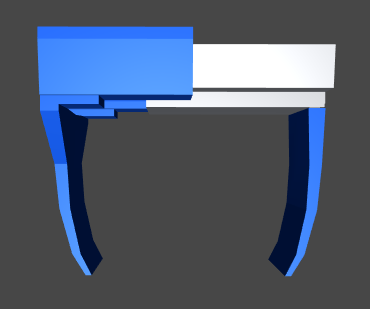
\includegraphics[width=\linewidth]{figures/gripper}
\caption{gripper}
\label{fig:gripper-sim}
\end{subfigure}%
    \hfill
\begin{subfigure}[t]{0.33\textwidth}
\centering
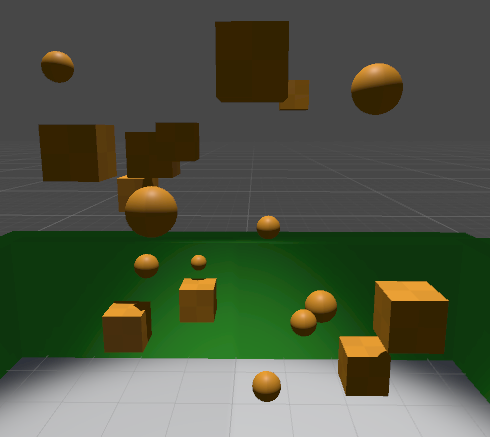
\includegraphics[width=\linewidth]{figures/obstructions}
\caption{obstructions}
\label{fig:obstructions-sim}
\end{subfigure}%
    \hfill
\begin{subfigure}[t]{0.33\textwidth}
\centering
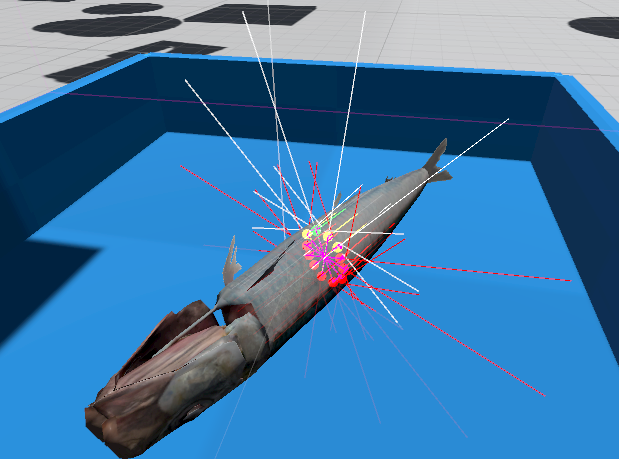
\includegraphics[width=\linewidth]{figures/target}
\caption{fish}
\label{fig:fish-sim}
\end{subfigure}%

\caption{In the problem enviroment 
(a) %\ref{fig:gripper-sim}
is the gripper that navigate the obstruction 
(b) %\ref{fig:obstructions} 
to the target fish 
(c)%\ref{fig:fish-sim}
.}
\label{fig:problem-environment}
\end{figure}

All material produced during the summer of 2017 for the Neodroid project is hosted at \url{https://github.com/sintefneodroid}, the source code is published under Apache License 2.0.